\chapter{Correlation plots of n$\sigma$ for different particle pairs}
\label{appendixB}
\FloatBarrier
\begin{figure}[ht]
    \centering
    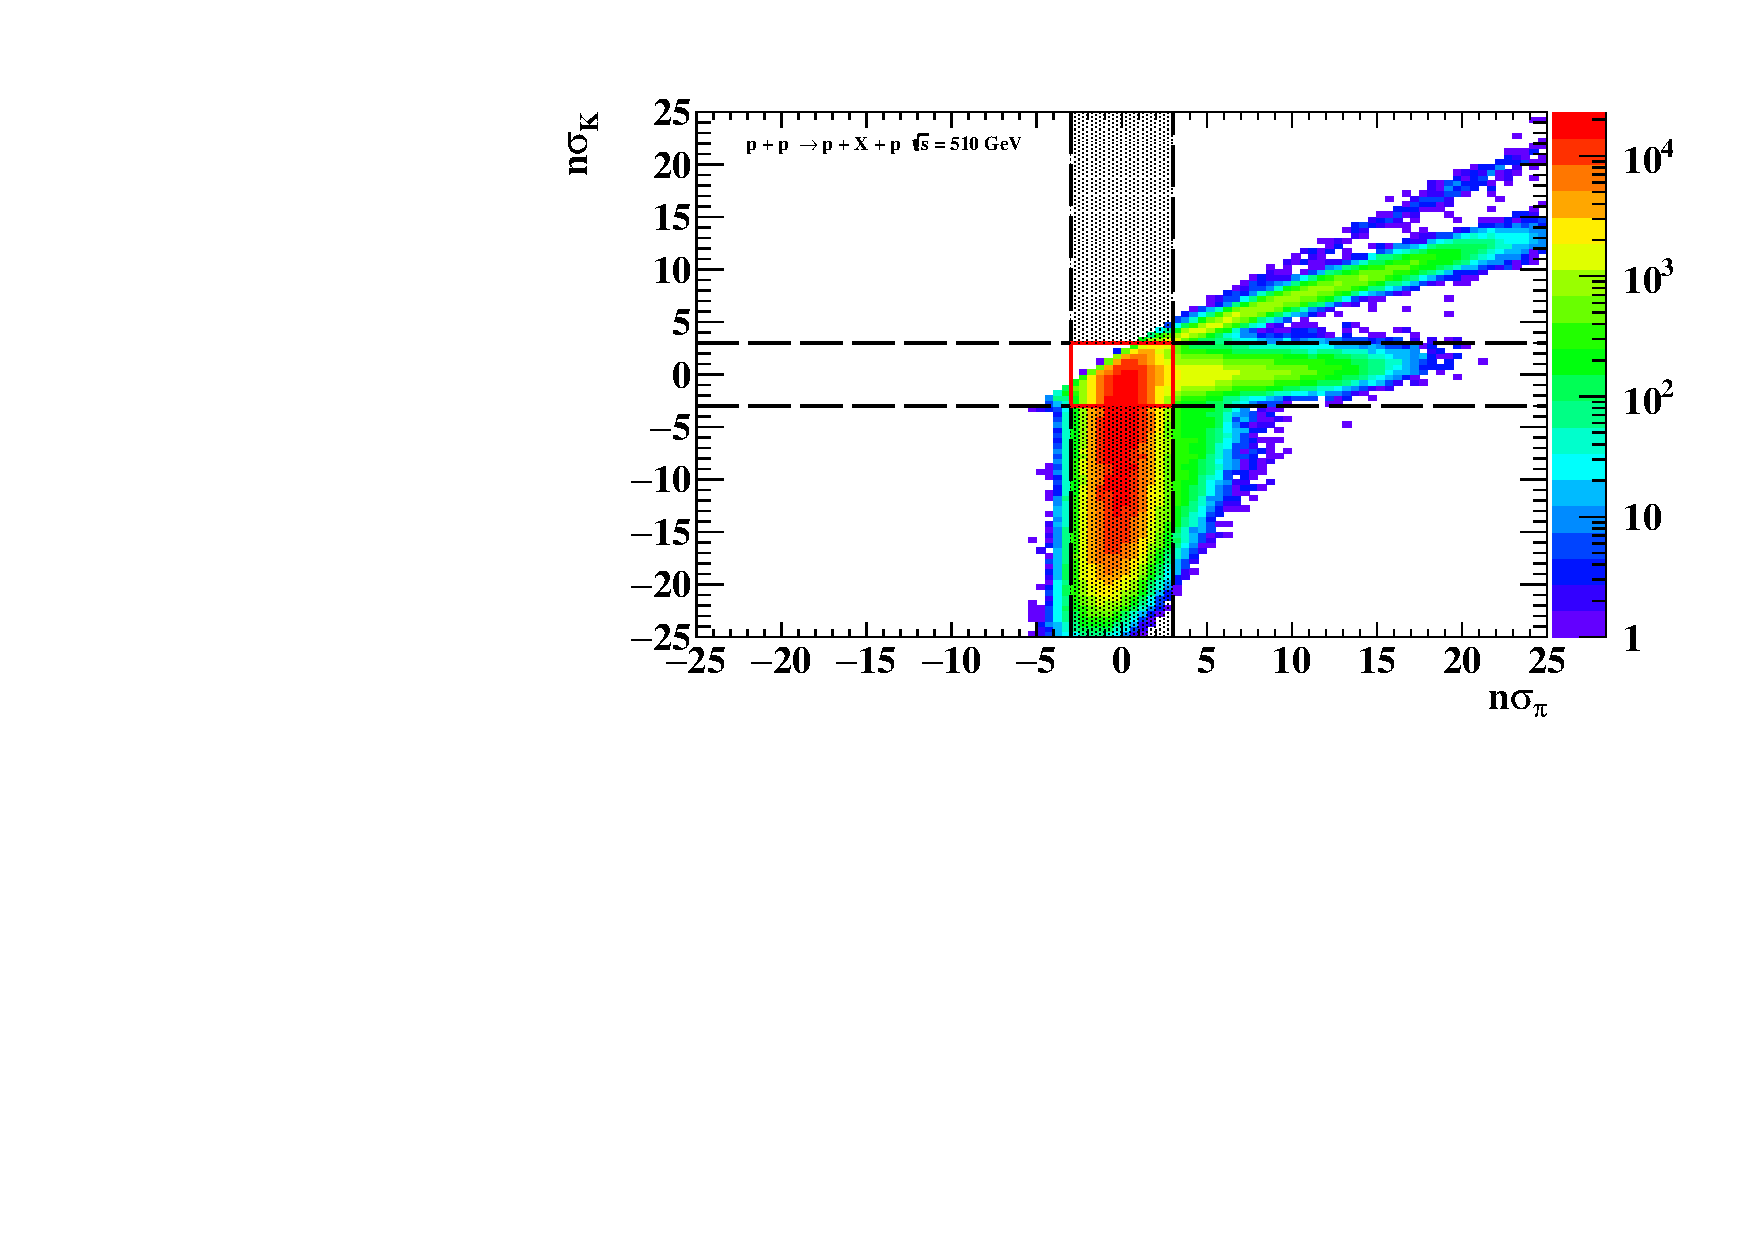
\includegraphics[width=1\textwidth]{figures/hNSigmaPiKcorr.pdf}
    \caption[Correlation graph of $n\sigma_{\pi}$ and $n\sigma_{K}$ of measured particles]{Correlation graph of $n_{\sigma}$ of pions on the $x$ axis and $n_{\sigma}$ for kaons on the $y$ axis. Black lines represent the conditions for identification and the red box in the middle the overlay.}
    \label{a1}
\end{figure}
\FloatBarrier

\FloatBarrier
\begin{figure}[ht]
    \centering
    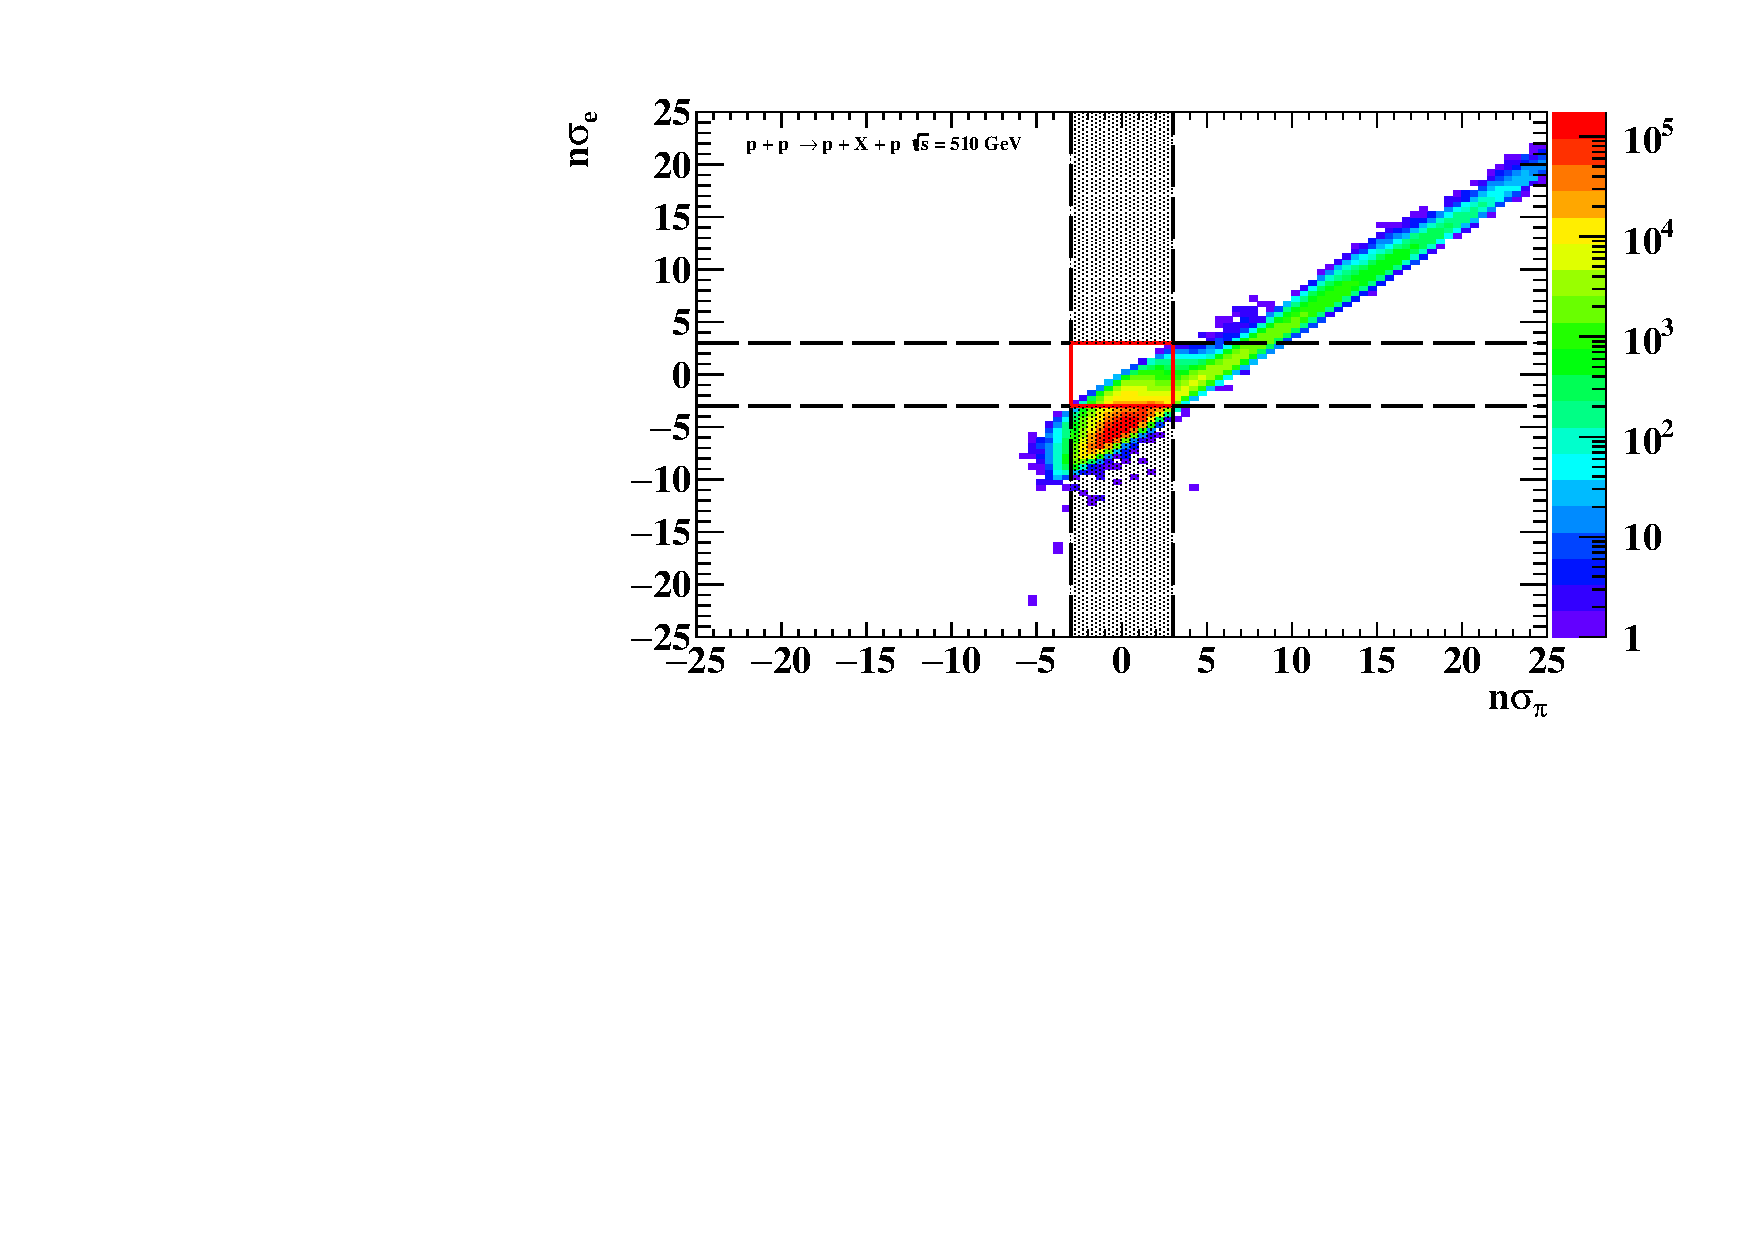
\includegraphics[width=1\textwidth]{figures/hNSigmaPiecorr.pdf}
    \caption[Correlation graph of $n\sigma_{\pi}$ and $n\sigma_{e}$ of measured particles]{Correlation graph of $n_{\sigma}$ for pions on the $x$ axis and $n_{\sigma}$ for electrons on the $y$ axis. Black lines represent the conditions for identification and the red box in the middle the overlay.}
    \label{a2}
\end{figure}
\FloatBarrier

\FloatBarrier
\begin{figure}[ht]
    \centering
    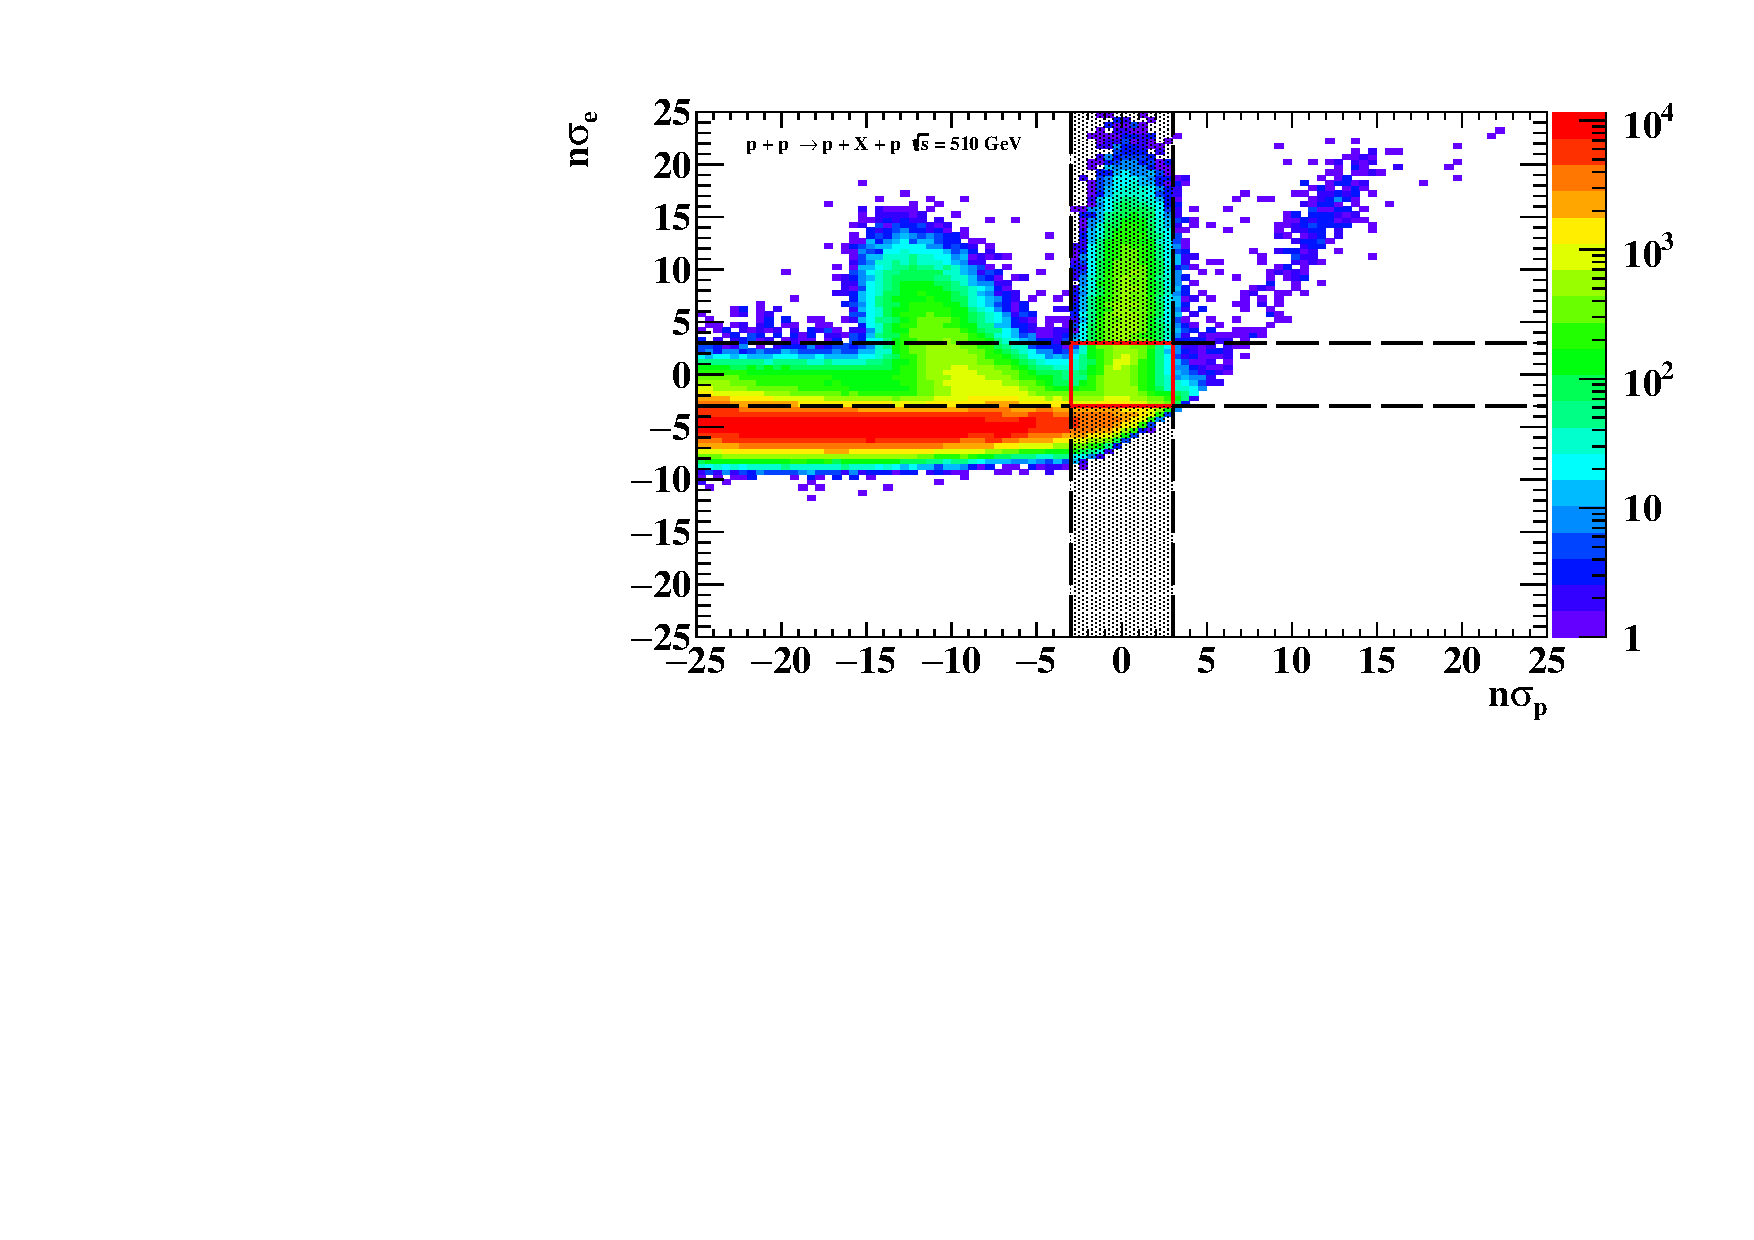
\includegraphics[width=1\textwidth]{figures/hNSigmaPecorr.pdf}
    \caption[Correlation graph of $n\sigma_{p}$ and $n\sigma_{e}$ of measured particles]{Correlation graph of $n_{\sigma}$ for protons on the $x$ axis and $n_{\sigma}$ for electrons on the $y$ axis. Black lines represent the conditions for identification and the red box in the middle the overlay.}
    \label{a3}
\end{figure}
\FloatBarrier

\FloatBarrier
\begin{figure}[ht]
    \centering
    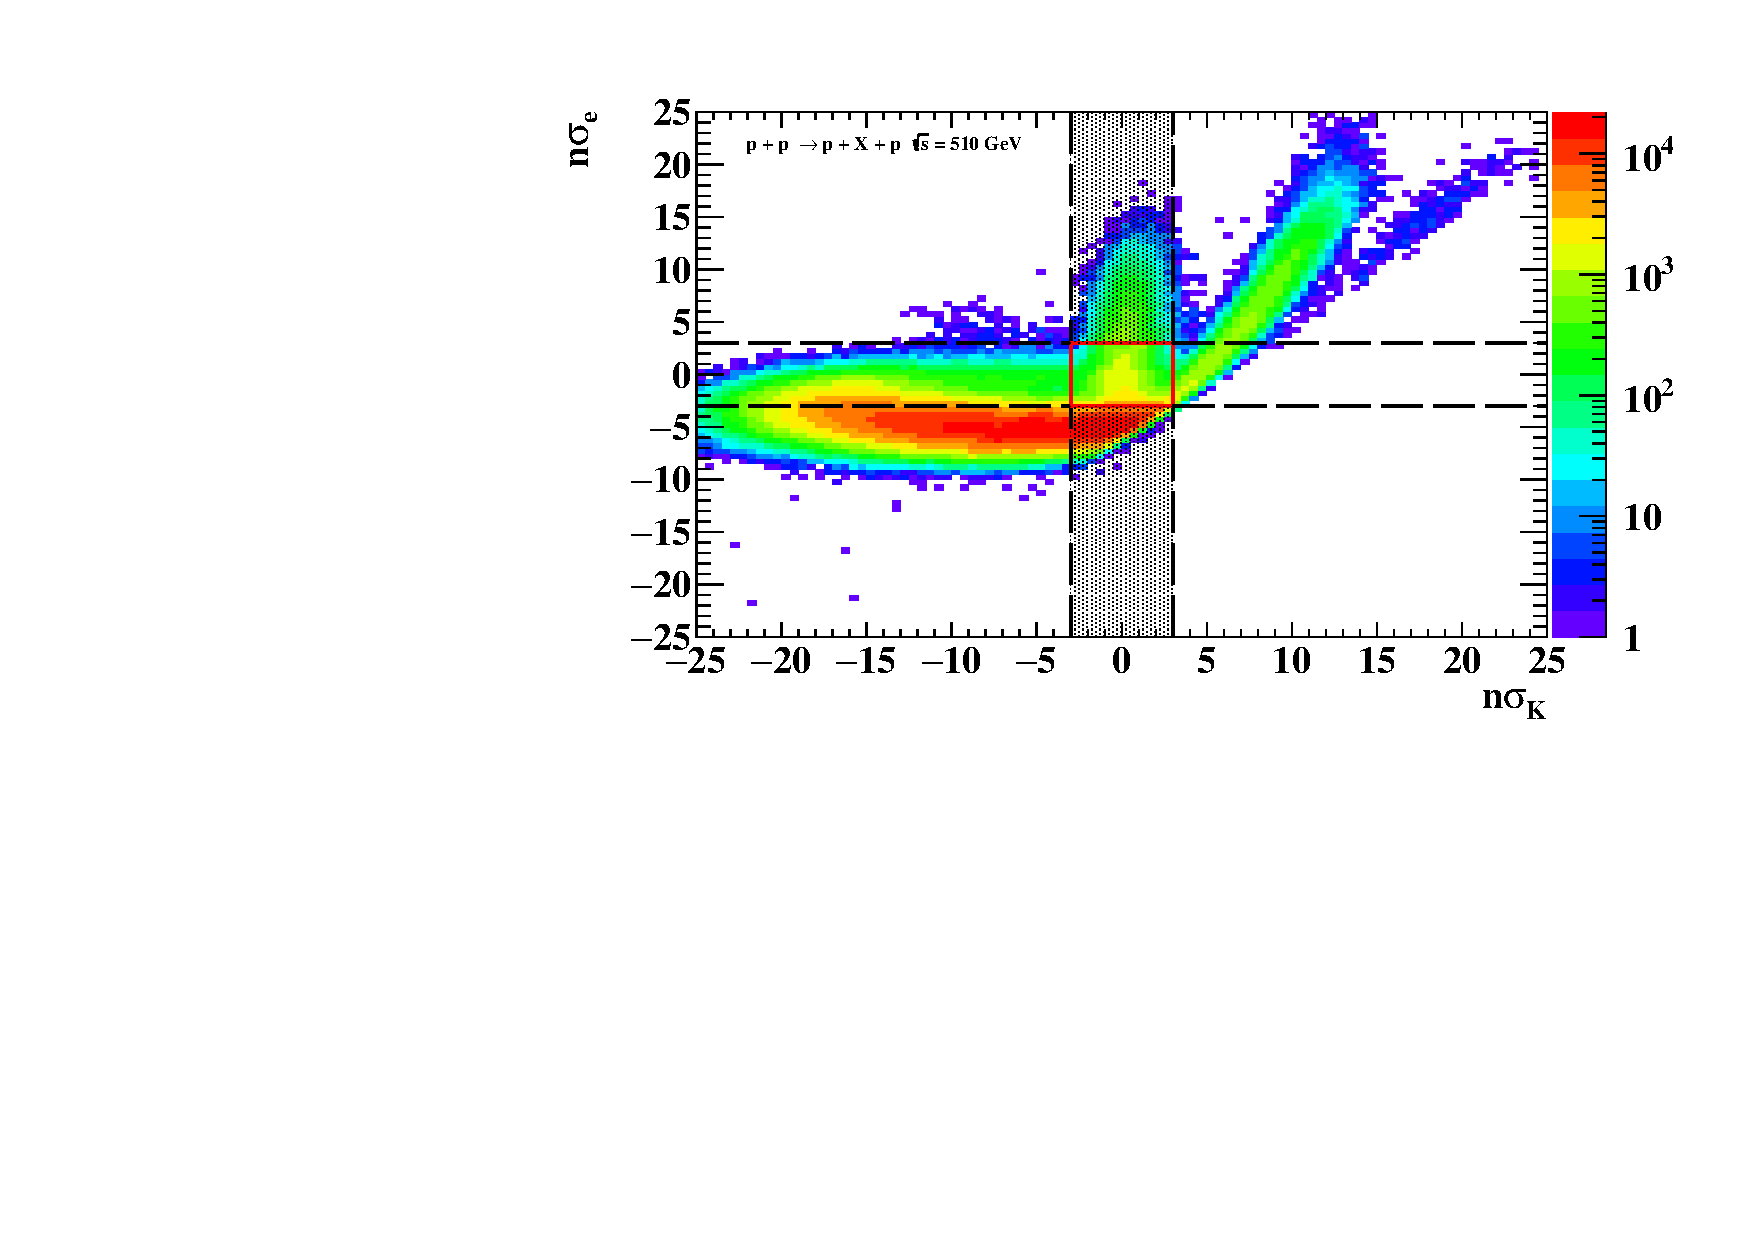
\includegraphics[width=1\textwidth]{figures/hNSigmaKecorr.pdf}
    \caption[Correlation graph of $n\sigma_{K}$ and $n\sigma_{e}$ of measured particles]{Correlation graph of $n_{\sigma}$ for kaons on the $x$ axis and $n_{\sigma}$ for electrons on the $y$ axis. Black lines represent the conditions for identification and the red box in the middle the overlay.}
    \label{a4}
\end{figure}
\FloatBarrier

\FloatBarrier
\begin{figure}[ht]
    \centering
    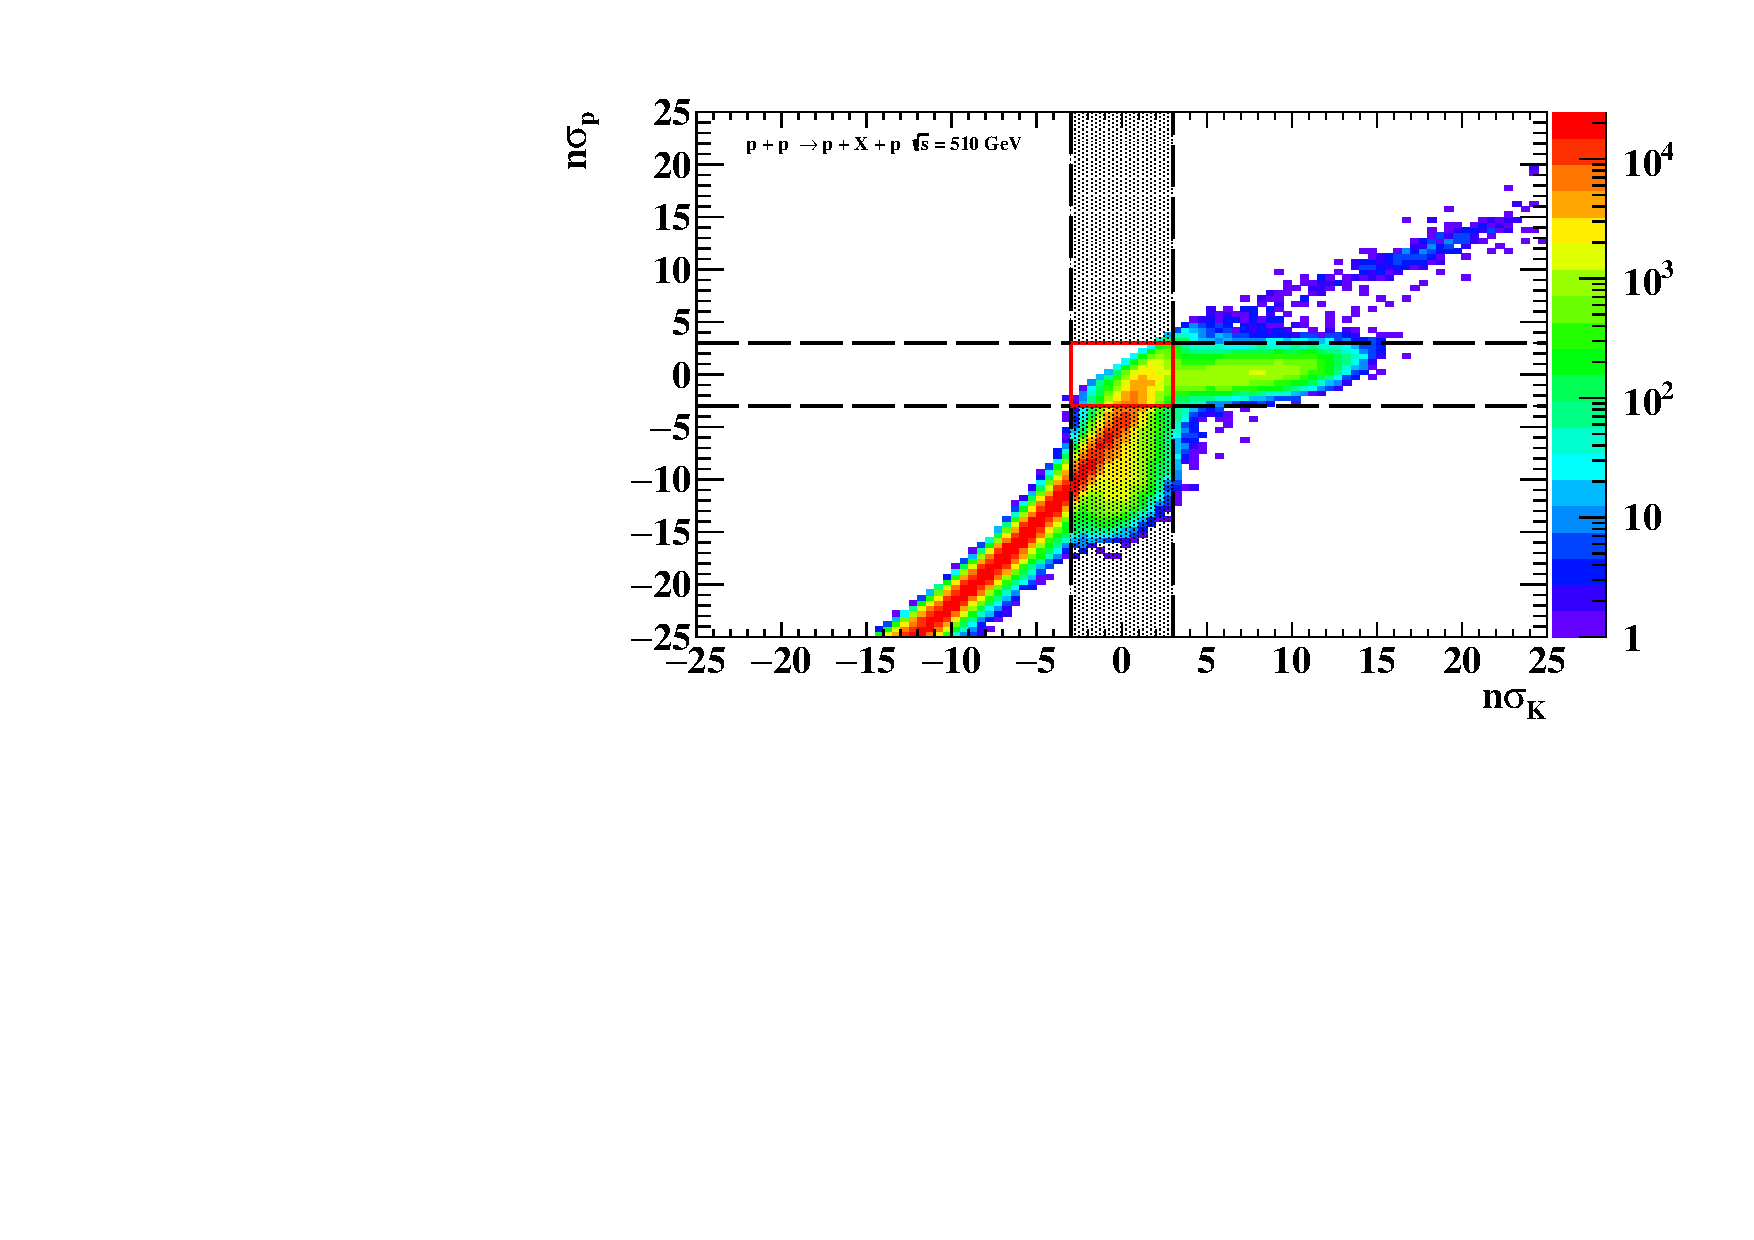
\includegraphics[width=1\textwidth]{figures/hNSigmaKPcorr.pdf}
    \caption[Correlation graph of $n\sigma_{K}$ and $n\sigma_{p}$ of measured particles]{Correlation graph of $n_{\sigma}$ for kaons on the $x$ axis and $n_{\sigma}$ for protons on the $y$ axis. Black lines represent the conditions for identification and the red box in the middle the overlay.}
    \label{a4}
\end{figure}
\FloatBarrier

\FloatBarrier
\begin{figure}[ht]
    \centering
    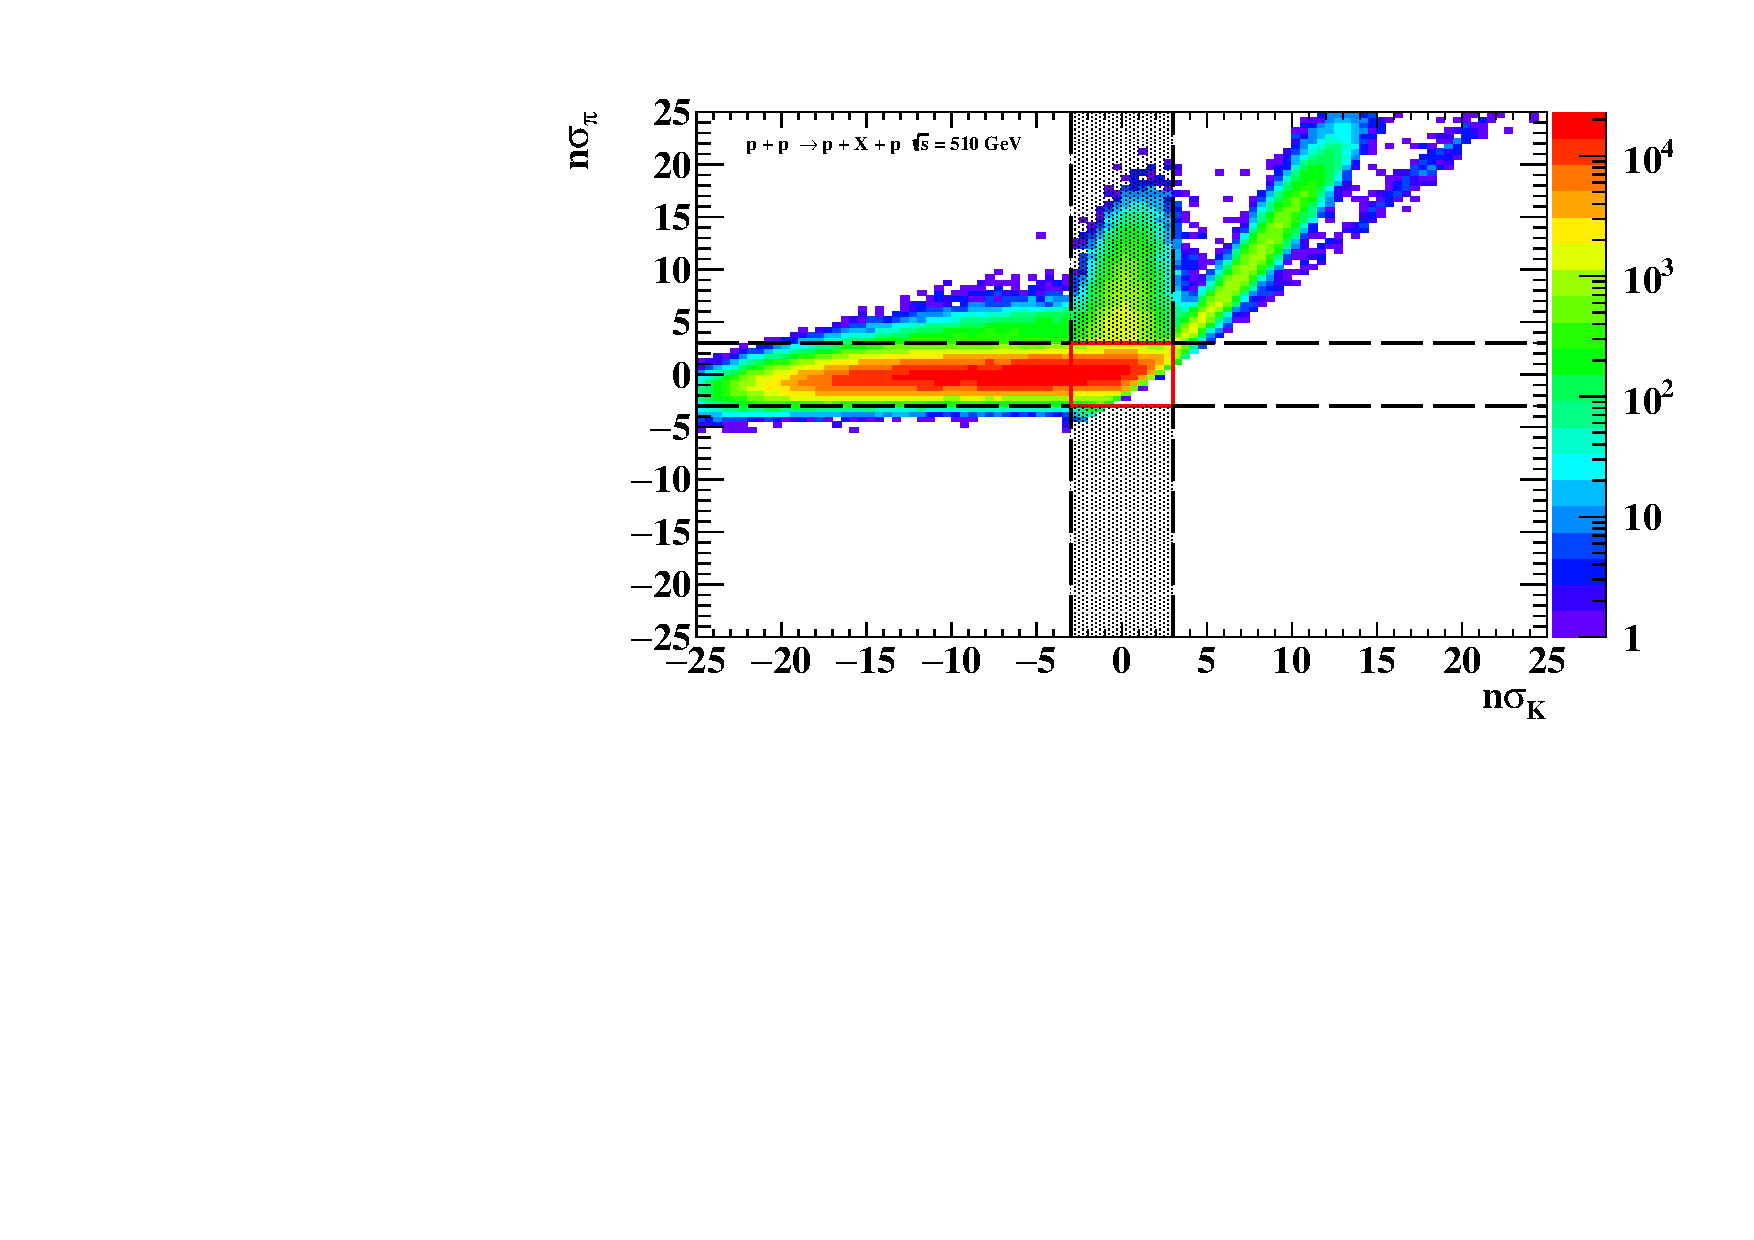
\includegraphics[width=1\textwidth]{figures/hNSigmaKPicorr.pdf}
    \caption[Correlation graph of $n\sigma_{K}$ and $n\sigma_{\pi}$ of measured particles]{Correlation graph of $n_{\sigma}$ for kaons on the $x$ axis and $n_{\sigma}$ for pions on the $y$ axis. Black lines represent the conditions for identification and the red box in the middle the overlay.}
    \label{a4}
\end{figure}
\FloatBarrier

\FloatBarrier
\begin{figure}[ht]
    \centering
    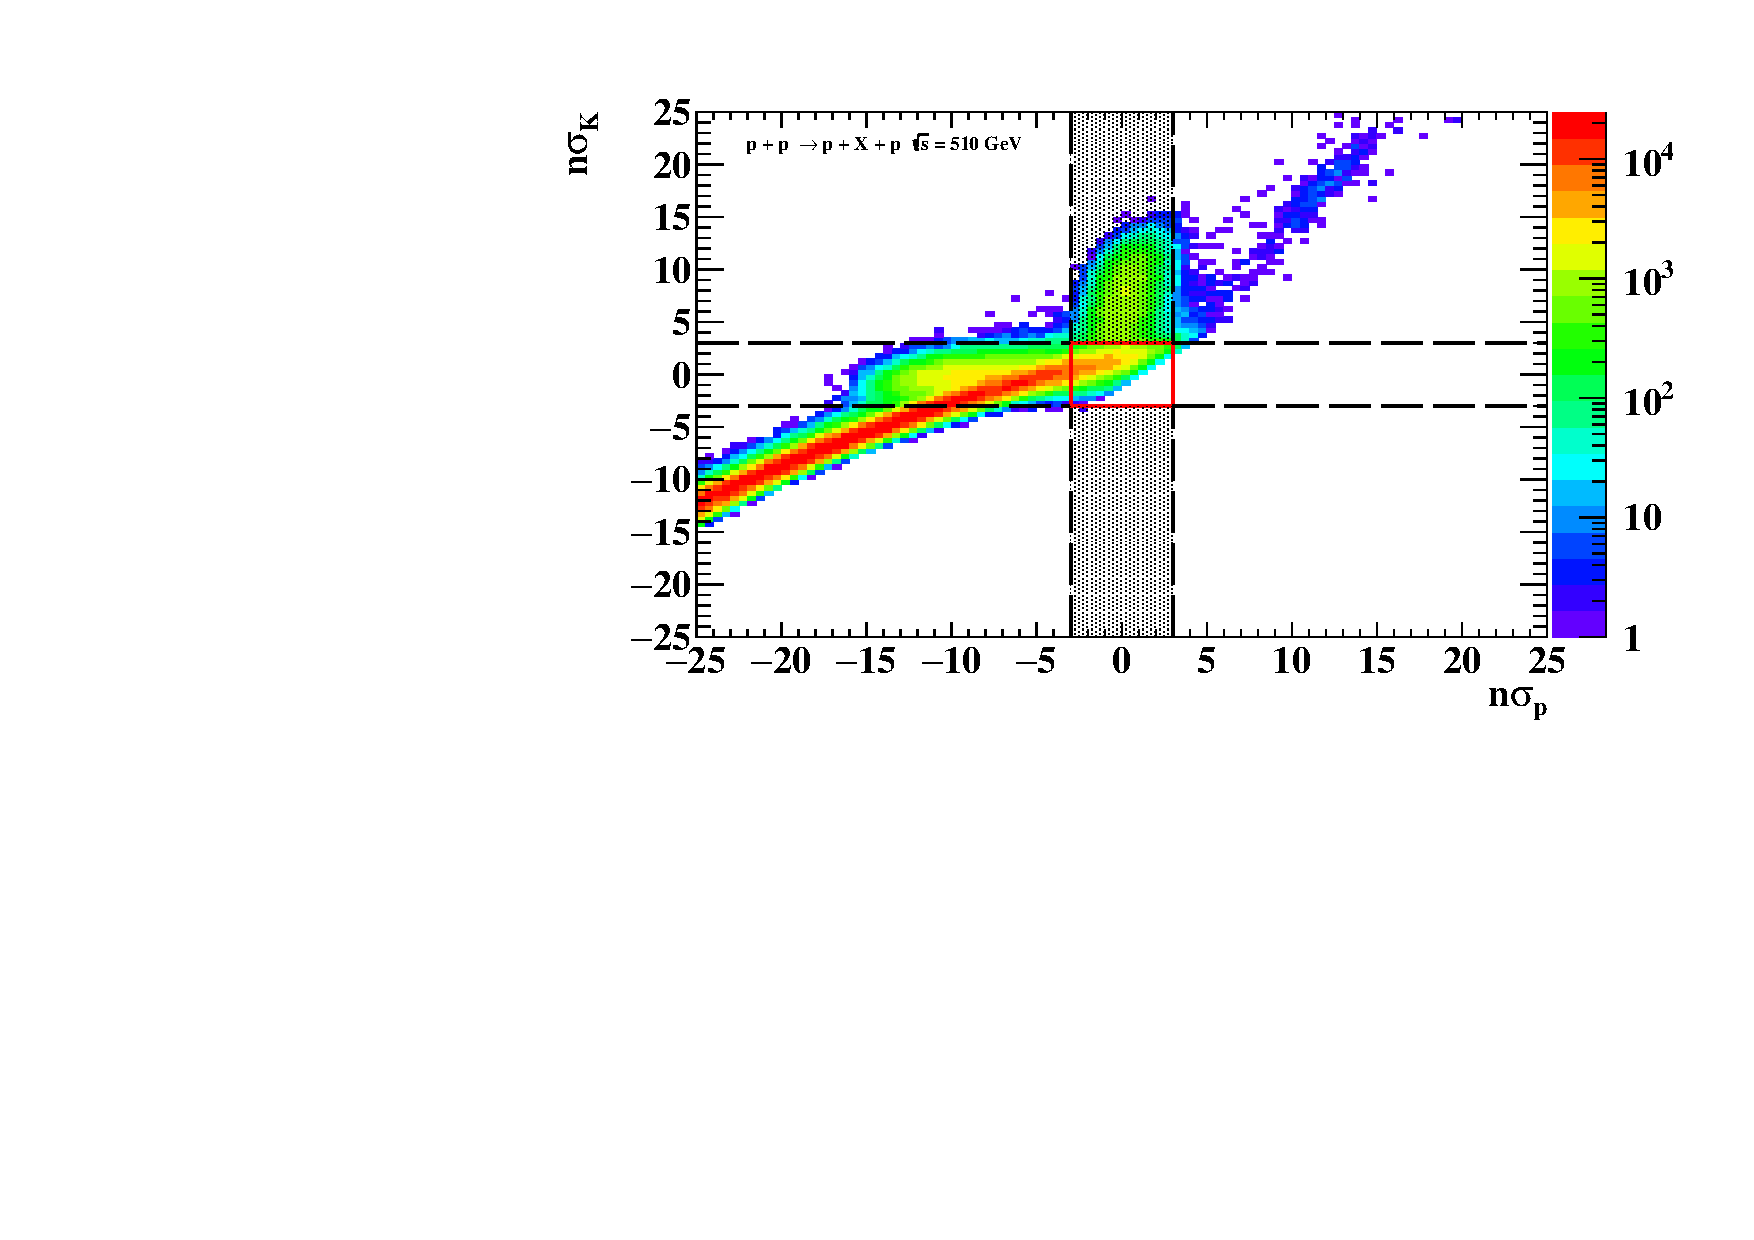
\includegraphics[width=1\textwidth]{figures/hNSigmaPKcorr.pdf}
    \caption[Correlation graph of $n\sigma_{p}$ and $n\sigma_{K}$ of measured particles]{Correlation graph of $n_{\sigma}$ for protons on the $x$ axis and $n_{\sigma}$ for kaons on the $y$ axis. Black lines represent the conditions for identification and the red box in the middle the overlay.}
    \label{a4}
\end{figure}
\FloatBarrier

\FloatBarrier
\begin{figure}[ht]
    \centering
    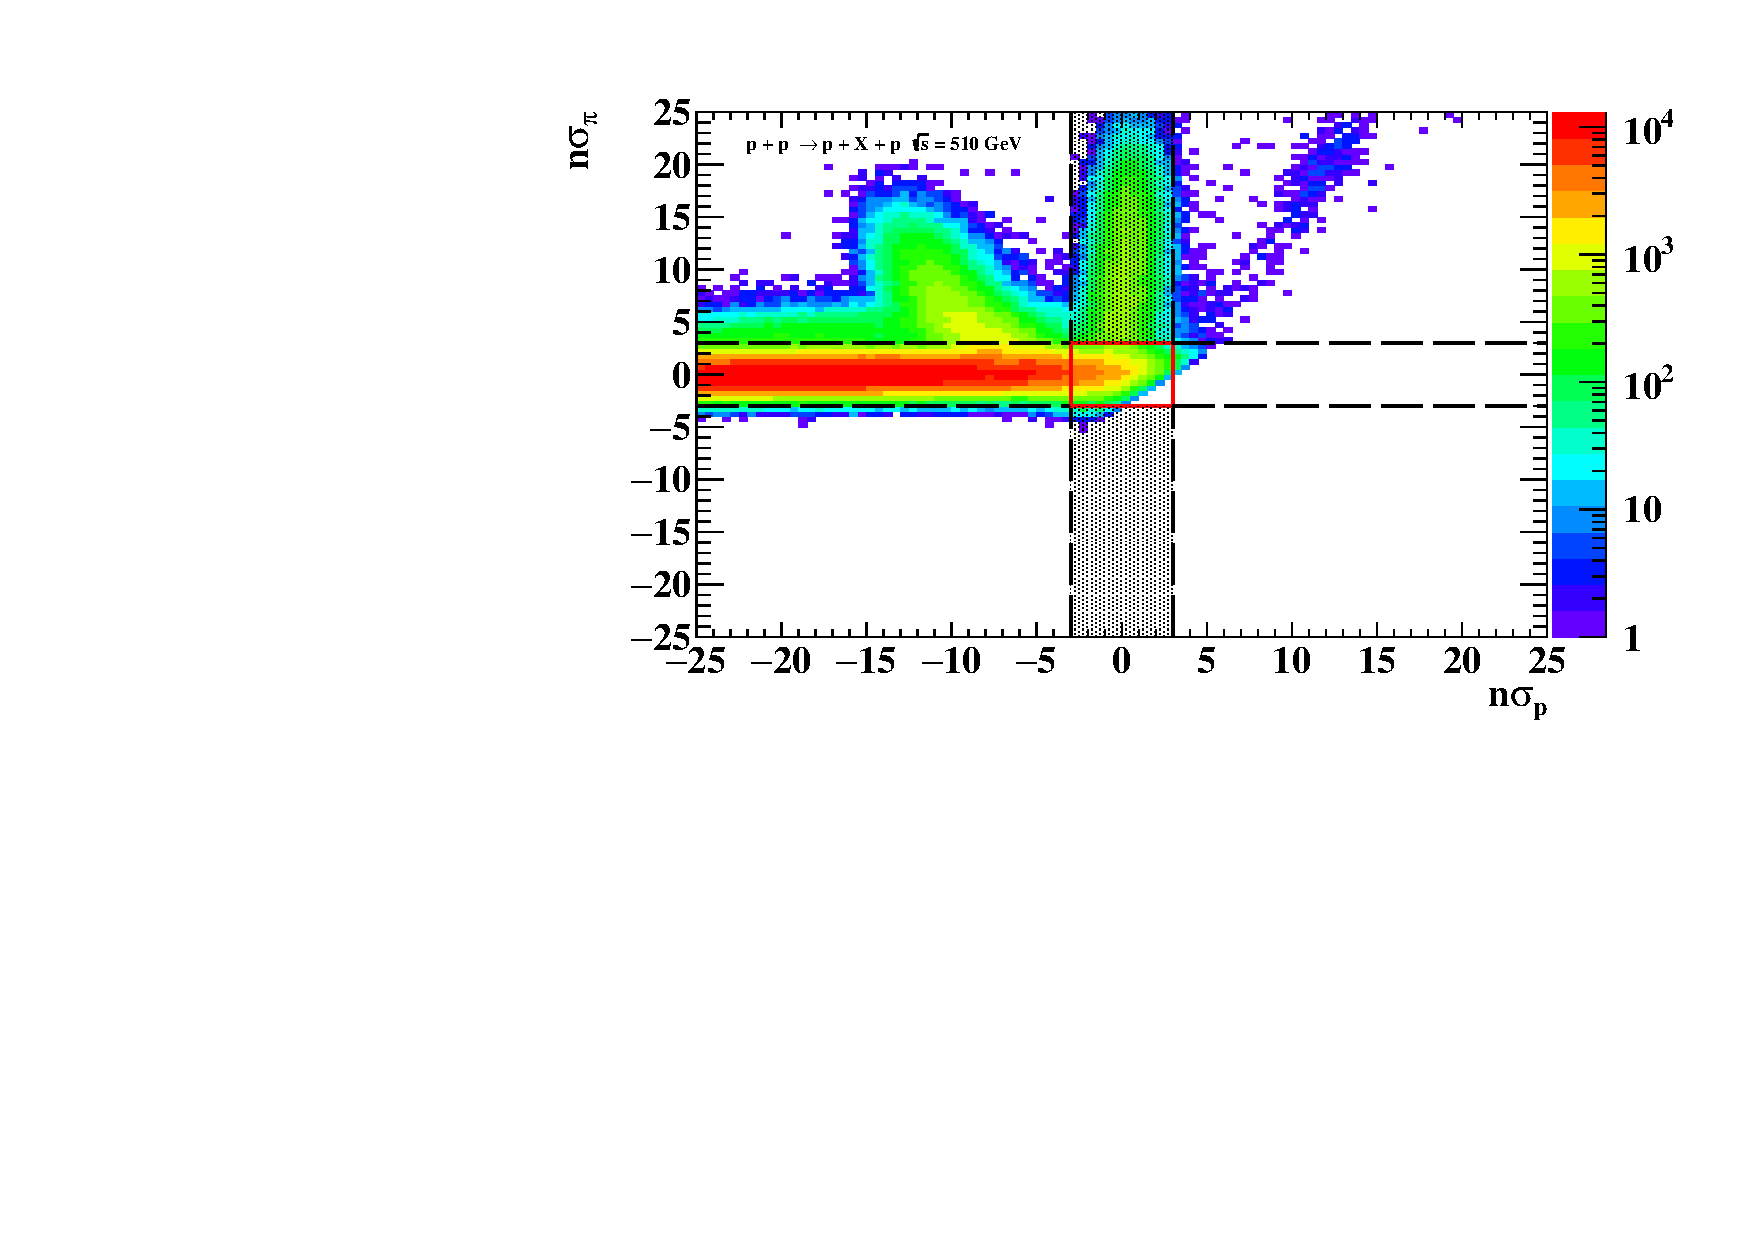
\includegraphics[width=1\textwidth]{figures/hNSigmaPPicorr.pdf}
    \caption[Correlation graph of $n\sigma_{p}$ and $n\sigma_{\pi}$ of measured particles]{Correlation graph of $n_{\sigma}$ for protons on the $x$ axis and $n_{\sigma}$ for pions on the $y$ axis. Black lines represent the conditions for identification and the red box in the middle the overlay.}
    \label{a4}
\end{figure}
\FloatBarrier
